\chapter{Introducción}\label{ch:introduction}

En los últimos años hemos visto como los smartphones se han convertido en un dispositivo esencial para cualquier persona. La mayoría de gente, entre los que me incluyo, no pueden salir de casa sin él. ¿Quién me iba a decir que hasta mis padres los utilizarían?. Este crecimiento en el uso de los smartphones ha propiciado la aparición dispositivos más o menos relacionados como tablets, smartwatches y Smart TV.

El desarrollo de todo este nuevo hardware ha traído consigo el desarrollo nuevo software. Desde sistemas operativos que controlan y dan vida a los dispositivos, a las aplicaciones que sacan partido a todo su potencial y son las que ofrecen al usuario nuevas funcionalidades que al final es lo que busca al comprar este tipo de terminales.

Un software que por otro lado no para de crecer, y que se tiene que adaptar a unos dispositivos que evolucionan a un ritmo desorbitado. Unos dispositivos que cada vez son más potentes y que cada vez incorporan nuevas características a las que poder sacar provecho, como por ejemplo, los sensores de huella dactilar que han surgido como medio de autenticación del usuario sustituyendo a las habituales contraseñas. El software también debe hacer frente a la variedad de usuarios que hacen uso de estos dispositivos y lo que esperan encontrar en estos. Aplicaciones para la oficina, videojuegos, realidad virtual, aplicaciones para el aprendizaje de idiomas, mensajería, \ldots un sinfín de tipos de aplicaciones que podemos encontrarnos hoy en día.

\begin{figure}[H]
\centering
  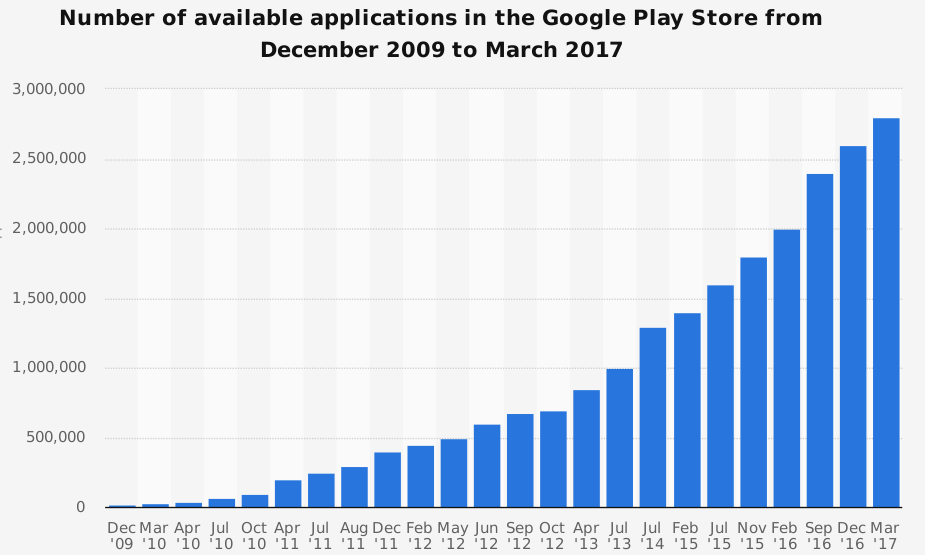
\includegraphics[width=0.8\textwidth]{Figures/ch1/introduction/google_play_number_of_apps}
  \caption{Crecimiento del número de aplicaciones disponibles en la tienda de Android, el sistema operativo para smartphones con más volumen de terminales en uso. \cite{GooglePlayApps}.}
\end{figure}

\section{Plataformas móviles: Android, iOS y el resto.}

Si dejamos a un lado la batalla entre los fabricantes de hardware (Samsung, LG, Sony, \ldots), nos encontramos con otra batalla en lo referente a la plataforma o sistema operativo utilizado.

En un principio, cada fabricante de teléfonos tenía su propio sistema operativo, el cual incluía en sus dispositivos. Además, eran los propios fabricantes los encargados de desarrollar las aplicaciones que se ejecutarían en sus terminales, lo que limitaba en gran medida la variedad de estás aplicaciones.

Mas tarde, diferentes fabricantes empezaron a unirse para crear conjuntamente sistemas operativos que compartían. El más famoso sin duda alguna fue Symbian. Este sistema operativo, propiedad de Nokia, fue producto de la alianza de esta con otras compañías como Siemens, Samsung, LG, \ldots pero fue Nokia la que más partido le saco y con la que se hizo famoso el sistema. Uno de los puntos fuertes de Symbian fue la gran comunidad de desarrolladores que realizaban aplicaciones para esta plataforma, lo que la hacía muy atractiva para un usuario final que, hasta entonces, apenas disponía de tonos y fondos de pantalla para personalizar su terminal.

Fue en 2007 cuando ocurrió un evento muy importante. La compañía Apple, ya famosa por sus ordenadores y su iPod, presento Iphone OS, que más tarde pasaría a llamarse \emph{iOS}, su nombre actual. Junto con el nuevo sistema aparecía el primer iPhone, el smartphone que sin duda supuso el inicio del \emph{boom} de este tipo de dispositivo. Este sistema es propietario de Apple, y solo lo podemos encontrar en sus terminales iPhone e iPad. Sus aplicaciones empezaron siendo escritas en Objective-C, lenguaje que años más tarde cambiaron para utilizar Switch. Este es un dato importante para lo que explicaremos a continuación.

Un año más tarde, allá por septiembre de 2008, Google presenta su sistema operativo, Android. Este sistema operativo estaba realizado por una empresa del mismo nombre, la cual Google había comprado unos años antes. La versión más básica es conocida como \gls{AOSP}, que se trata de un proyecto de código abierto. A diferencia de iOS, podremos encontrar Android en multitud de dispositivos de multitud de fabricantes, desde smartphones a encontrarse instalado en sistemas multimedia para automóviles, desde Samsung a BQ. En el caso de Android las aplicaciones están escritas usando Java.

El carácter abierto de Android ha propiciado que aparezcan diversos firmwares basados en él. Quizás los más conocidos sean MIUI\footnote{\url{http://en.miui.com/}}, propio de los terminales de Xiaomi, y el ya descontinuado CyanogenMOD. Pero por la web, podemos encontrar multitud de versiones y personalizaciones del sistema creada por la comunidad de desarrolladores. También es común que los fabricantes de smartphones que usen Android, creen su propia versión personalizada de este.

Junto a estos dos sistemas operativo han convivido otros como el ya mencionado Symbia, Windows y BlackBerry (que tuvo una época dorada allá por 2008). También intentos menos exitosos, como Fire OS de Amazon, Firefox OS (basado en HTML5) o Ubuntu Touch de Canonical. Pero si algo tienen en común todos ellos, es que se han convertido, o no han pasado de serlo, en sistemas operativos residuales en cuanto a cuota de mercado. En la siguiente tabla podemos ver esta cuota en el tercer cuatrimestre de 2016.

\begin{figure}[H]
\centering
  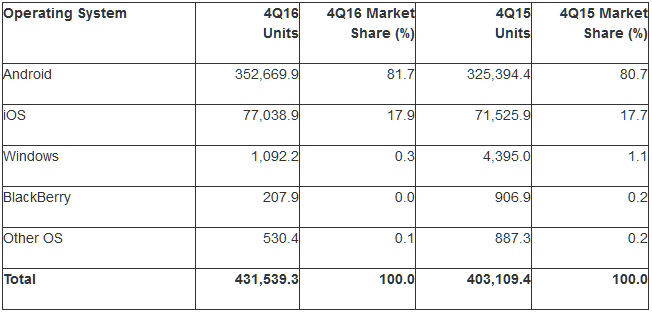
\includegraphics[width=\textwidth]{Figures/ch1/introduction/smartphone_sales_3q_2016}
  \caption{Cuota de mercado en el cuarto cuatrimestre del año 2016 según la plataforma. \cite{SmartPhonesSales}.}
\end{figure}

Otro dato curioso para ver la importancia que han tomado estos sistemas operativos y este tipo de dispositivos, es comparar el número de dispositivos conectados  a internet según su sistema operativo a lo largo del tiempo. En la siguiente gráfica se puede ver como peso de Windows para PC disminuye en tanto que el de los sistemas operativos para terminales móviles crecen.

\begin{figure}[H]
\centering
  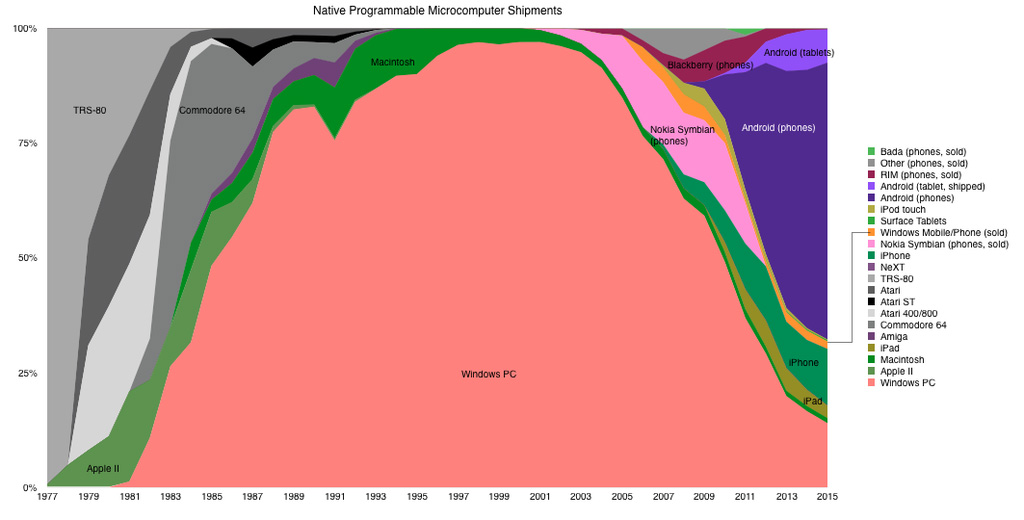
\includegraphics[width=\textwidth]{Figures/ch1/introduction/os_quota}
  \caption{Distribución de los dispositivos conectados a internet teniendo en cuenta el sistema operativo que utilizan.  \cite{PlatformsWar}. }
\end{figure}

\subsection{¿Un nuevo contendiente?. Google Fuchsia.}

\cite{Fuchsia} En el momento de escribir esta memoria (10 de mayo de 2017), se filtrado el que posiblemente sea un nuevo sistema operativo creado por Google. Este sistema vendría a unificar los dos sistemas operativos de la compañía, Android y Chrome OS\footnote{\url{https://www.chromium.org/chromium-os}}.

Las mayores características de este nuevo sistema serian por un lado, el abandono del kernel de linux del que hacen uso tanto Android como Chrome OS. Este sería remplazado por un kernel desarrollado por Google y que responde al nombre de Magenta. La otra diferencia sería el uso de Flutter SDK\footnote{\url{https://flutter.io/}}, un \gls{SDK} también desarrollado por Google para la creación de aplicaciones multiplataforma que se centra en el rendimiento y que utiliza el lenguaje Dart\footnote{\url{https://www.dartlang.org/}} (una alternativa a JavaScript lanzada por Google). Este \gls{SDK} aun se encuentra en sus primeras fases de desarrollo, pero de ser usado en el nuevo sistema, significaría que las aplicaciones creadas para Fuchsia, podrían ser también usadas en Android. En la web de Flutter SDK podemos encontrar una aplicación no funcional válida para Android en la que podemos ver una pequeña muestra de la UI que ofrece, la cual es conocida con el nombre de Armadillo.

Aun es pronto para saber los planes que tiene Google con este sistema operativo, y que hará con Android. Pero podemos encontrarnos con que en un futuro próximo se una esta nueva plataforma a Android y a iOS, diversificando más el mercado. Y es que aunque Google apueste por el nuevo sistema, serán los fabricantes de smartphone los que tendrán que introducirlos en sus dispositivos, y como se comento anteriormente, muchos de ellos cuentan con versiones personalizadas. Esto hará que el paso de Android a Fuchsia (en el caso de que se produzca) se alargue en el tiempo y ambas plataformas convivan.

\section{En la variedad está problema. Aplicaciones híbridas.}

A la hora de implementar una aplicación nos encontramos con el dilema de, ¿a qué dispositivo va dirigido?. Viendo las cuotas de mercado, se podría pensar que la opción mejor es lanzarse a crear nuestra aplicación para Android. Pero si investigamos un poco, veremos que las aplicaciones lanzadas en iOS producen hasta cuatro veces más beneficios que las de Android \cite{AndroidiOSRevenue}. Por otro lado, lo más probable es que no nos interese desarrollarla solo para iOS ya que Android cuenta con 7 veces más usuarios. También tenemos que pensar en la función que va a tener nuestra aplicación. Si por ejemplo, nuestra aplicación se basa en recoger datos de cualquier tipo (por ejemplo, reportar accidentes de tráfico) y compartirlos entre usuarios de la aplicación, nos interesa que nuestra aplicación llegue al mayor número de usuarios posible para poder captar un volumen mayor de datos. O si nuestra aplicación forma parte de un producto, como puede ser manejar un drone, no podemos excluir a una parte de potenciales compradores del producto únicamente por no disponer de un terminal que le permita ejecutar nuestra aplicación. Y no nos olvidemos de Windows \ldots

Como vemos, parece más que recomendable abarcar al menos las dos plataformas mas importantes a la hora de crear una aplicación, pero no siempre se cuenta con los recursos o conocimientos necesarios para abordar dos proyectos diferentes y no solo eso, si no también mantenerlos.

Para solventar este problema surgieron las \emph{aplicaciones híbridas}, ¿para qué programar dos aplicaciones desde cero si van a tener un mismo funcionamiento?. Mientras que las \emph{aplicaciones nativas} se desarrollan en el lenguaje específico de cada plataforma y utilizando la \gls{API} propia de cada sistema, las aplicaciones híbridas utilizan tecnología web (HTML5, CSS y JavaScript) para crear la aplicación y a continuación, mediante el uso de diferentes herramientas, son compiladas lo que genera un ejecutable para cada una de las plataformas.

Las aplicaciones hibridas nos ofrecen ventajas sobre las nativas, pero también presentan sus desventajas. En internet se pueden encontrar multitud de comparativas entre ambos tipos de aplicaciones y según el autor, las diferencias entre ellas serán mas o menos importantes. aún así, a continuación expondré aquellos puntos que considero más importantes a la hora de decidir por que tipo de aplicación apostar.

\paragraph{Curva de aprendizaje} En el caso de las aplicaciones nativas, debemos aprender como funcionan estas en cada una de las plataformas, el lenguaje que se utiliza para programar, las APIs que ofrece el sistema, \ldots en cambio, para las aplicaciones híbridas, solo será necesario saber HTML, CSS y JS junto con el framework o herramientas que utilicemos para ayudarnos a crear nuestras aplicación. Además, los frameworks que han aparecido para ayudar en la creación de aplicaciones híbridas facilitan mucho el trabajo con algunas de las \glspl{API} del sistema operativo, llegando a ser más fácil utilizarlas a través del framework, que de manera nativa. Este es el punto fuerte de las aplicaciones híbridas.

\paragraph{Diseño de la aplicación} Aunque cada vez son más y mejores los frameworks que nos ayudan a crear las aplicaciones híbridas, es cierto que en el desarrollo de este tipo de aplicaciones es más complicado el tener un diseño acorde a la plataforma. Puede parecer un problema menor, pero el aspecto de una aplicación es muy importante, y la experiencia de uso puede verse perjudicada al utilizar ciertos estilos a los que el usuario no esta acostumbrado (widgets, botones, distribución de elementos, \ldots). El problema puede ser aún mayor si la aplicación esta destinada para iOS, ya que Apple puede vetarla de su market si no cumple con ciertos estándares de diseño.

Puede parecer desproporcionado este énfasis en cuanto a la homogeneidad del diseño, pero si pensamos en los ordenadores de sobremesa, ocurre lo mismo. Por ejemplo, los usuarios de Windows estamos acostumbrados a que los botones para minimizar/cerrar una ventana se encuentren en la esquina superior derecha y sería complicado adaptarse a que eso no fuera así. Solo hay que ver las críticas que recibió Microsoft cuando lanzo Windows 8 con su menú, teniendo que volver a uno más tradicional en la versión 8.1.

\paragraph{Rendimiento de la aplicación} Otro punto en contra de las aplicaciones híbridas es el rendimiento. Suelen mostrarse más lentas que las nativas. Este problema puede no ser crítico en función del tipo de aplicación y si tenemos en cuenta que cada vez los dispositivos móviles son más potentes. Aun así, es un punto a tener en cuenta.

\paragraph{Seguriad} Por norma general, las aplicaciones nativas son más seguras que las hibridas. No nos olvidemos que estas últimas suelen hacer uso de frameworks que en su mayoría son libres y su código es abierto, lo que facilita la búsqueda de debilidades. Esto hace que su uso sesa poco recomendable en aplicaciones sensible, como por ejemplo aquellas que gestionen cuentas bancarias.

\paragraph{Disponibilidad de las capacidades del terminal} Es posible que no tengamos acceso (o esté limitado) a ciertas capacidades del dispositivo, por ejemplo, algún sensor en concreto, desde una aplicación híbrida. Evidentemente, este problema no lo tendremos con una aplicación nativa. Es por tanto importante comprobar que la tecnología que elijamos cubra nuestras necesidades, y no encontrarnos con esta limitación a mitad del desarrollo lo que conllevaría un esfuerzo extra \textbf{MUY} importante.

\paragraph{Costes} El factor que suele tener (lamentablemente) más peso a la hora de elegir. Es evidente que, una aplicación hibrida tiene un menor coste, ya que no requiere el dedicar un equipo de trabajo para cada plataforma. Incluso teniendo que implementar la aplicación para solo una, es muy posible que la aplicación híbrida sea una opción más económica (y deja la puerta abierta a ser lanzada en otras plataformas en el futuro).

En resumen, las aplicaciones hibridas son una buena alternativa para la mayoría de aplicaciones de hoy en día, y con la evolución de los framework, cada vez más. Pero si queremos una aplicación robusta, con una interfaz cuidada y un rendimiento óptimo, y siempre que el presupuesto lo permita, la opción nativa sigue siendo la más indicada.

Una buena estrategia es utilizar aplicaciones híbridas en la etapa inicial de nuestro proyecto y según cómo responda el mercado a nuestra idea, decidirse a dar el paso y hacer el cambio a aplicaciones nativas, eso sí, siempre que sea necesario.

\subsubsection{Frameworks al rescate}

Para ayudar al desarrollo de aplicaciones hibridas han surgido frameworks que facilitan la tarea de integración de las diferentes plataformas haciendo que converjan en una única interfaz.

Sin duda alguna, el proyecto que más ha impulsado la creación de aplicaciones híbridas  ese a sido Adobe Cordova (como veremos más adelante, también conocido como PhoneGap), que proporcionan las herramientas necesarias para que nuestra aplicación basada en tecnología web pueda ser ejecutada en el dispositivo. Junto con Cordova, han aparecido multitud de frameworks, algunos de los cuales utilizan Cordova como base, los cuales facilitan el desarrollo ofreciendo conjuntos de componentes estéticos, añadiendo patrones de programación, potenciando las tecnologías web usadas (\gls{HTML}, \gls{CSS} y \gls{JS}), \ldots.
